\section{Job-scheduling}

In this type of game we investigate on a situation in which we have a
multi-core CPU and a number of tasks queued to be executed. We are not
concerned with avoiding starvation anymore: now the focus is having the
lowest cost of execution, which in different terms means to spread the
load (the tasks) as evenly as possible throughout all of the cores. By
cost, we mean time.

The threads of execution are now running in parallel, and they can
choose which core they want to use. If more than 1 thread chooses the
same core, the payoff for each task will be worse: in fact the core will
take more time to complete each task. Obviously we want to reduce the
likelihood of many threads competing for a single core.

What we are after is simulating a generic CPU scheduler for a multi-core
CPU: a CPU scheduler is an entity that has complete control over the
execution of threads.

In this game each task has full knowledge over the environment, each
task is selfish and wants to complete as fast as possible, and knows
that all other processes wants the same: in a real operating system
tasks have no knowledge of their surrounding environment, they only
communicate with threads from the same process, but this is a reasonable
abstraction, since we want to simulate a game where actually the CPU
scheduler makes every decision, and the CPU scheduler knows the global
context.

A congestion game fits well this
situation: it is a game where the set of players \(N\) consume resources
from the set \(M\). The set of strategies for player \(i\in N\) is
denoted by \(S_i\), where \(s_i \in S_i\), and \(s_i\) is a non-empty
subset of \(M\). Call \(s = \{s_1,...,s_n\}\) a strategy profile. For
\(j\in M\), \(c_j\in \mathbb{R}^n\) is a vector of costs, where
\(c_j(k)\) is the cost related to each user of the resource \(j\), if
there are \(k\) players using that resource.

The overall cost function for player \(i\) is
\(u_i(s_i, s_{-i})=\sum_{j\in s_i} c_j(n_j(s_i, s_{-i}))\), where the
notation \(s_{-i}\) means all players' strategies except for \(i\)'s. We
define \(n_j(s)\) as the number of players using the resource
\(j\in M\).

A job-scheduling game is a special type of congestion game called
singleton congestion game: each player can select only a single
resource, thus we can simplify the game as follows:

\begin{itemize}
\item
  \(N = \{1..n\}\) is the set of players, namely the threads of
  execution
\item
  \(M = \{1..m\}\) is the set of resources, the cores of the CPU
\item
  \(S_i\) is the set of strategies for player \(i\in N\) and
  \(s_i\in M\), if \(s_i = j\) it means that thread \(i\) uses core
  \(j\)
\item
  \(n_j(s)\) is a function \(n_j:M^n\rightarrow\mathbb{N}\), that given
  a strategy profile \(s\) returns the current cost for core \(j\).
\end{itemize}

Note that we suppose that cores and threads are heterogeneous,
respectively. This means that all threads are equal, and a thread using
a core has the same cost as any other thread using the same core.

For example, if the cost of using a core is \(k\), and there are exactly
\(x\) players using the core \(j\) then the overall cost for using such
resource is simply \(k \cdot x\). The generic overall cost function for
player \(i\) can then be simplified to:

\[ u_i(s)= k \cdot n_{s_i}(s) \]

\begin{center}
% generated by Plantuml 1.2022.7       
\definecolor{plantucolor0000}{RGB}{24,24,24}
\definecolor{plantucolor0001}{RGB}{0,0,0}
\definecolor{plantucolor0002}{RGB}{144,238,144}
\scalebox{.6}{%
\begin{tikzpicture}[yscale=-1
,pstyle0/.style={color=plantucolor0000,line width=1.0pt}
,pstyle1/.style={color=plantucolor0000,fill=black,line width=0.5pt}
,pstyle2/.style={color=plantucolor0000,fill=plantucolor0002,line width=0.5pt}
,pstyle3/.style={color=plantucolor0000,fill=plantucolor0000,line width=1.0pt}
]
\draw[pstyle0] (60pt,218pt) arc (180:270:36pt) -- (96pt,182pt) -- (180pt,182pt) arc (270:360:36pt) -- (216pt,218pt) -- (216pt,218pt) arc (0:90:36pt) -- (180pt,254pt) -- (96pt,254pt) arc (90:180:36pt) -- (60pt,218pt) -- cycle;
\node at (129.8857pt,189pt)[below right,color=black]{\textbf{M}};
\draw[pstyle0] (7pt,69pt) arc (180:270:62pt) -- (69pt,7pt) -- (243pt,7pt) arc (270:360:62pt) -- (305pt,69pt) -- (305pt,69pt) arc (0:90:62pt) -- (243pt,131pt) -- (69pt,131pt) arc (90:180:62pt) -- (7pt,69pt) -- cycle;
\node at (148.9667pt,14pt)[below right,color=black]{\textbf{N}};
\draw[pstyle1] (138pt,229pt) ellipse (8pt and 8pt);
\node at (113.3163pt,246pt)[below right,color=black]{$m_1$};
\draw[pstyle1] (191pt,229pt) ellipse (8pt and 8pt);
\node at (179.9077pt,246pt)[below right,color=black]{$m_2$};
\draw[pstyle1] (85pt,229pt) ellipse (8pt and 8pt);
\node at (73.9077pt,246pt)[below right,color=black]{$m_3$};
\draw[pstyle2] (138pt,80pt) ellipse (8pt and 8pt);
\node at (129.4444pt,97pt)[below right,color=black]{$n_1$};
\draw[pstyle2] (209pt,80pt) ellipse (8pt and 8pt);
\node at (200.4444pt,97pt)[below right,color=black]{$n_2$};
\draw[pstyle2] (85pt,80pt) ellipse (8pt and 8pt);
\node at (76.4444pt,97pt)[below right,color=black]{$n_3$};
\draw[pstyle2] (280pt,80pt) ellipse (8pt and 8pt);
\node at (271.4444pt,97pt)[below right,color=black]{$n_4$};
\draw[pstyle2] (32pt,80pt) ellipse (8pt and 8pt);
\node at (23.4444pt,97pt)[below right,color=black]{$n_5$};
\draw[pstyle0] (138pt,89.32pt) ..controls (138pt,113.38pt) and (138pt,183.2pt) .. (138pt,213.59pt);
\draw[pstyle3] (138pt,218.25pt) -- (142pt,209.25pt) -- (138pt,213.25pt) -- (134pt,209.25pt) -- (138pt,218.25pt) -- cycle;
\node at (139pt,148pt)[below right,color=black]{k};
\draw[pstyle0] (205.18pt,88.9pt) ..controls (193.73pt,112.62pt) and (159.53pt,183.42pt) .. (144.84pt,213.85pt);
\draw[pstyle3] (142.67pt,218.33pt) -- (150.1838pt,211.9627pt) -- (144.8429pt,213.8269pt) -- (142.9788pt,208.486pt) -- (142.67pt,218.33pt) -- cycle;
\node at (176pt,148pt)[below right,color=black]{k};
\draw[pstyle0] (85pt,89.32pt) ..controls (85pt,113.38pt) and (85pt,183.2pt) .. (85pt,213.59pt);
\draw[pstyle3] (85pt,218.25pt) -- (89pt,209.25pt) -- (85pt,213.25pt) -- (81pt,209.25pt) -- (85pt,218.25pt) -- cycle;
\node at (86pt,148pt)[below right,color=black]{k};
\draw[pstyle0] (276.94pt,89.12pt) ..controls (272.5pt,100.56pt) and (263.74pt,121.94pt) .. (254pt,139pt) ..controls (237.84pt,167.31pt) and (214.92pt,197.8pt) .. (201.64pt,214.73pt);
\draw[pstyle3] (198.79pt,218.34pt) -- (207.5052pt,213.7526pt) -- (201.8873pt,214.4149pt) -- (201.225pt,208.7969pt) -- (198.79pt,218.34pt) -- cycle;
\node at (248pt,148pt)[below right,color=black]{k};
\draw[pstyle0] (35pt,89.32pt) ..controls (43.71pt,113.48pt) and (69.06pt,183.78pt) .. (79.94pt,213.97pt);
\draw[pstyle3] (81.52pt,218.34pt) -- (82.2467pt,208.518pt) -- (79.832pt,213.6336pt) -- (74.7164pt,211.2188pt) -- (81.52pt,218.34pt) -- cycle;
\node at (63pt,148pt)[below right,color=black]{k};
\end{tikzpicture}}
\captionof{figure}{Represents a strategy profile of a singleton congestion game, where the players $n_i$ compete for a resource $m_j$.}
\label{fig:jobSchedulingExample}
\end{center}

Figure \ref{fig:jobSchedulingExample} represents a job-scheduling game.

We define the following typical solution of a job-scheduling game:

\begin{itemize}
\item
  the Nash equilibrium, is a strategy profile \(s^*\) such that
  \(u_i(s^*)\leq u_i(s_i, s^*_{-i})\), for all \(i\in N\), for all
  \(s_i\in S_i\)
\item
  the Pareto optimal solution, a strategy profile \(\bar{s}\) such that
  \(\nexists s\) with \(u_i(s)\leq u_i(\bar{s})\) for each \(i\in N\)
  and \(u_i(s)< u_i(\bar{s})\) for at least one \(i\in N\).
\end{itemize}

Paper \cite{10.1145/1807406.1807411} defines a type of pareto optimality called social
optimum: a strategy profile such that \(\min \sum_{i\in N} u_i(s)\).
Interestingly enough, in our simple congestion game, any Nash
equilibrium is a social optimum. This property shows that even though
the threads are chasing only their own interest a Pareto optimal
solution is still reached.

\section{Job-scheduling repeated game}

We represented a one-shot static game where a round of the game shows a
decision of the scheduler. In this section we study what happens if we
play many rounds of this game. 
The game has the following properties:
\begin{itemize}
  \item each player wants to minimize the average
  cost over time
  \item each player knows the outcome of each one of the
  previous games
  \item we do not consider a discount for this type of game.
\end{itemize}

we suppose that each thread has the same duration \(d\), we can solve
the repeated game through backwards induction.

What if \(d\) is not known? Then the threads a way to solve this
repeated game is to suppose the game to be infinite.

The one-shot job scheduling game can evolve in a slightly different way
depending on the following situations:

\begin{enumerate}
\def\labelenumi{\arabic{enumi}.}
\item
  \(|N| \leq |M|\)
\item
  \(|N| \geq |M|\) \(|N| - \lfloor \dfrac{|N|}{|M|} \rfloor = 0\)
\item
  \(|N| \geq |M|\) and \(|N| - \lfloor \dfrac{|N|}{|M|} \rfloor > 0\).
\end{enumerate}

In both situation 1, 2 clearly there are more than one Nash equilibria,
since there are many possible distributions of threads across cores.
Weird situations may arise when we are in situation 2, and there are a
number of threads and cores such that
\(|N| - \lfloor \dfrac{|N|}{|M|} \rfloor > 0\): every core would like to
be executed by the core(s) which handle less threads, in order to reduce
their cost.

For the repeated game when the parameters respect 1, 2 no player would
want to deviate from a Nash equilibrium since all Nash equilibriums
yields the same payoff for each player.

Of course the CPU scheduler does not care about which Nash equilibrium
is played, since the global goal is to minimize the total cost.
For that reason, in situation 3, if the scheduler simply chooses a 
Nash equilibrium each round, while it will reach its global goal of minimizing
the cost, there might be a group of threads that have worse average payoff compared
to the others.

Since there is no immediate cooperation strategies such as tit-for-tat 
or grim trigger wouldn't work: what is a punishment, and what is a cooperative
strategy? 

Take for example the one-shot static game represented in figure \ref{fig:jobSchedulingRepeated}:
all strategies, except all threads choosing the same core are Nash equilibria, and
choosing any of such strategies would lead to an optimal play from the scheduler stand
point, but playing always $c_1$, $c_1$, $c_2$ for threads $t_1$, $t_2$, $t_3$ wouldn't
yield to a worse cost average for threads $t_1$, $t_2$. In order to avoid this situation
a possible strategy for the scheduler would be to switch to a different Nash equilibrium.

\begin{center}
  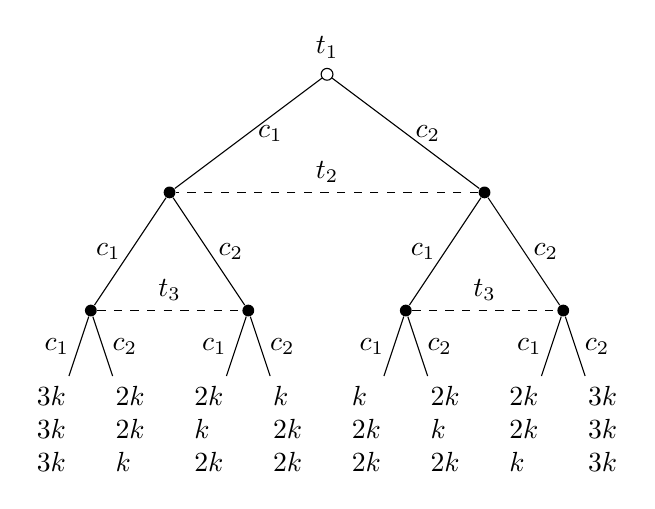
\begin{tikzpicture}[thin,
    level 1/.style={sibling distance=40mm},
    level 2/.style={sibling distance=20mm},
    level 3/.style={sibling distance=10mm},
    every circle node/.style={minimum size=1.5mm,inner sep=0mm}]
    
    \node[circle,draw,label=above:$t_1$] (root) {}
    child { node [circle,fill] (node-F) {}
    child { 
      node[circle,fill] (node-A) {}
        child {
          node[align=left] {$3k$\\$3k$\\$3k$}
          edge from parent
            node[left] {$c_1$}}
        child {
           node[align=left] {$2k$\\$2k$\\$k$}
           edge from parent
             node[right, align=left] {$c_2$}}
        edge from parent
          node[left] {$c_1$}}
    child { 
      node[circle,fill] (node-B) {}
        child {
          node[align=left] {$2k$\\$k$\\$2k$}
          edge from parent
            node[left] {$c_1$}}
        child {
          node[align=left] {$k$\\$2k$\\$2k$}
           edge from parent
             node[right] {$c_2$}}
        edge from parent
          node[right] {$c_2$}}
     edge from parent
       node[right] {$c_1$}}
      child { node [circle,fill] (node-E){}
        child { 
          node[circle,fill] (node-C) {}
            child {
              node[align=left] {$k$\\$2k$\\$2k$}
              edge from parent
                node[left] {$c_1$}}
            child {
              node[align=left] {$2k$\\$k$\\$2k$}
               edge from parent
                 node[right] {$c_2$}}
            edge from parent
              node[left] {$c_1$}}
        child { 
          node[circle,fill] (node-D) {}
            child {
              node[align=left] {$2k$\\$2k$\\$k$}
              edge from parent
                node[left] {$c_1$}}
            child {
              node[align=left] {$3k$\\$3k$\\$3k$}
               edge from parent
                 node[right] {$c_2$}}
            edge from parent
              node[right] {$c_2$}}
         edge from parent
           node[right] {$c_2$}};
    \draw [dashed] (node-C) -- (node-D) 
       node[midway,above] {$t_3$};
    \draw [dashed] (node-A) -- (node-B) 
       node[midway,above] {$t_3$};
    \draw [dashed] (node-E) -- (node-F) 
       node[midway,above] {$t_2$};
    \
  \end{tikzpicture}
  \captionof{figure}{Represents a job-scheduling game with 3 threads and 2 cores.}
  \label{fig:jobSchedulingRepeated}
  \end{center}